

% Chapter 

\chapter{Empirical Analysis : Insights from Stylized Facts} % Chapter title

\label{ch:empirical} % For referencing the chapter elsewhere, use \autoref{ch:name} 

%----------------------------------------------------------------------------------------


\headercit{Mais ce n'est pas une question d'{\^a}ge, de chiffres et de stats\\ Moi je te parle surtout de rage, de kif et d'espoir}{Youssoupha}{\textit{, Esperance de Vie}}





%  plan : 

%  1) static morphological analysis : requires a formal link between temporal and spatial correlations ?  -- typology etc can already be interesting --


%  2) presentation of BP case study

%  3) base Bien

%  4) Work with Solène



%----------------------------------------------------------------------------------------


As this quote suggests, a purely quantitative view of the world makes no sense without qualitative counterbalancing. More precisely, we argue that the \textit{clich{\'e}} of an opposition between quantitative and qualitative analysis is an illusion. No distinct boundary exists between both. We propose to call quantitative any process involving computation by a Turing machine, whereas the qualitative will be for us the modeling design process and its interpretations. Therefore both are necessarily closely interlaced in any of our approaches. In particular concerning the construction and the validation or refutation of our theory, empirical analysis on real case studies, implying the extraction and qualification of stylized facts, follows that schema.


We propose in this chapter various empirical analysis on different objects at different scales.
% articulation with theoretical questions
% articulation with modeling


%----------------------------------------------------------------------------------------


%%%%%%%%
%  Section : static analysis
%%%%%%%%

\newpage

\section{Static correlations of urban form and network shape}


Spatio-temporal processes implying diffusion or propagation phenomena generally have a specific structure of correlation. In particular, as derived in section~\ref{sec:spatiotempcorrs}, a static computation of correlation between different instances of a system may under certain conditions provide information on dynamical correlations implied.


% justify scale studied here


%%%%%%%%%%%%%%%%%%
\subsection{Morphological Measures of European Population Density}

\subsubsection{Context}

At the macroscopic scale of system of cities, spatialization of the urban system is reasonably captured by cities position, associated with aggregated city variable to represent entirely the system (see e.g. ontologies of Simpop models~\cite{pumain2012multi} or its successor Marius~\cite{cottineau2014evolution}). At the mesoscopic scale at which we aim to capture morphological manifestations of interactions between transportation networks and territories, structure of the territorial system can be specified by more refined indicators for the morphological aspect. 
% biblio spatial structure etc Florent

\subsubsection{Empirical Analysis}

We study systematically morphological indicators for constant size areas covering European Community. The choice of fixed size areas can be questioned regarding definition of a territorial system, that can be otherwise understood as a consistent spatial entity at a given scale and along certain criteria : \emph{Human territories} as defined by Raffestin (op. cit.) or more generally functionally autonomous spaces\footnote{for example, a tentative of definition of a \textit{Parisian} territory would present many facets. From the subjective territory point of view, intra-muros Parisians consider a strict boundary at \textit{Boulevard Periph{\'e}rique}, whereas close and even further suburbs will be seen as Parisians from the Province. The functional territory of \textit{Metropolitain} extends slightly further than the administrative boundary. Governance perimeters are currently mutating with the Metropolitan governance project. Complementary perceptions of the territory can thus be multiplied.}.





%%%%%%%%%%%%%%%%%%
\begin{figure}
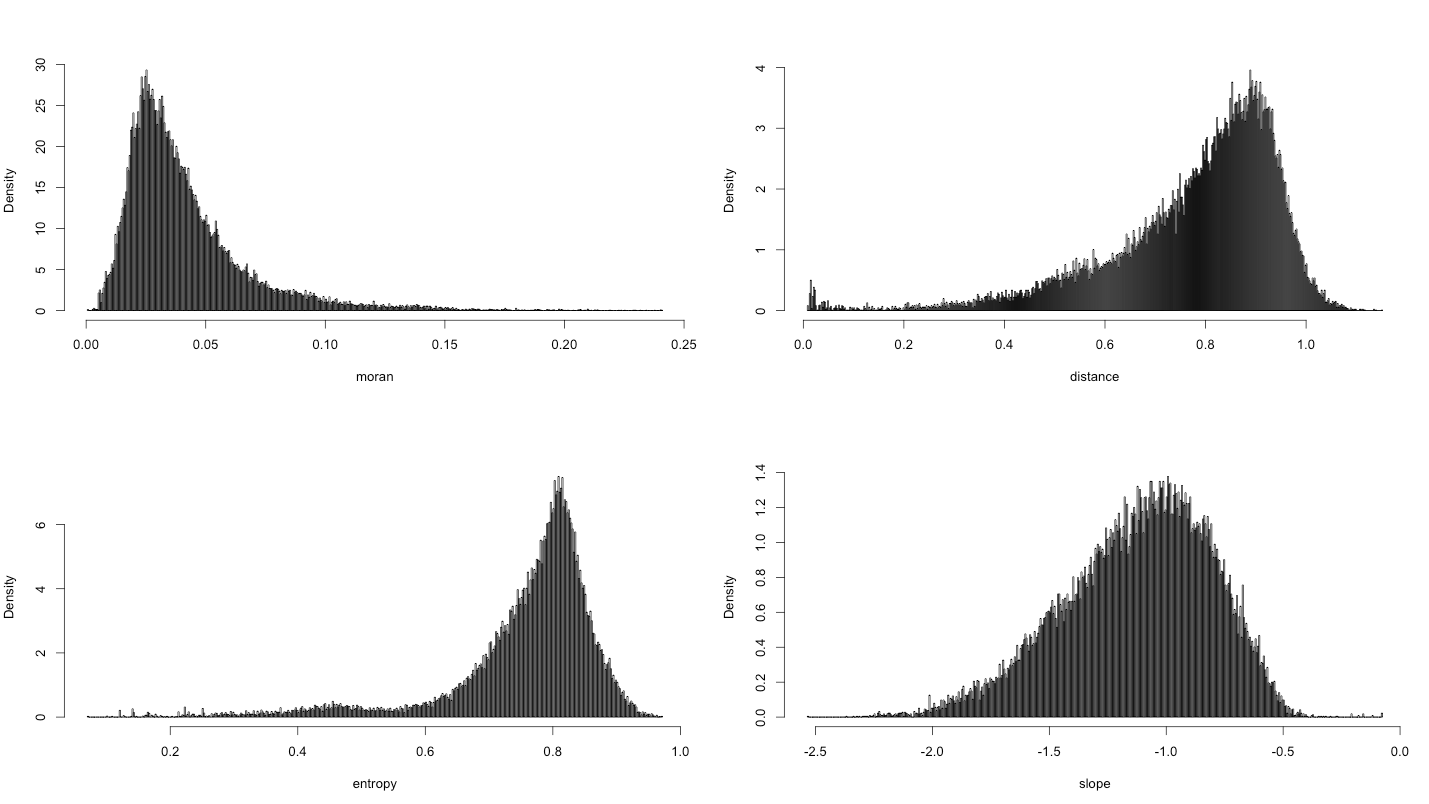
\includegraphics[width=1.2\textwidth]{Figures/PartII/Empirical/Static/Density/hists_GOOD}
\caption[Empirical Distribution of Morphological Indicators]{Empirical Distribution of Morphological Indicators}
\end{figure}
%%%%%%%%%%%%%%%%%%

%%%%%%%%%%%%%%%%%%
\begin{figure}
\hspace{-5cm}
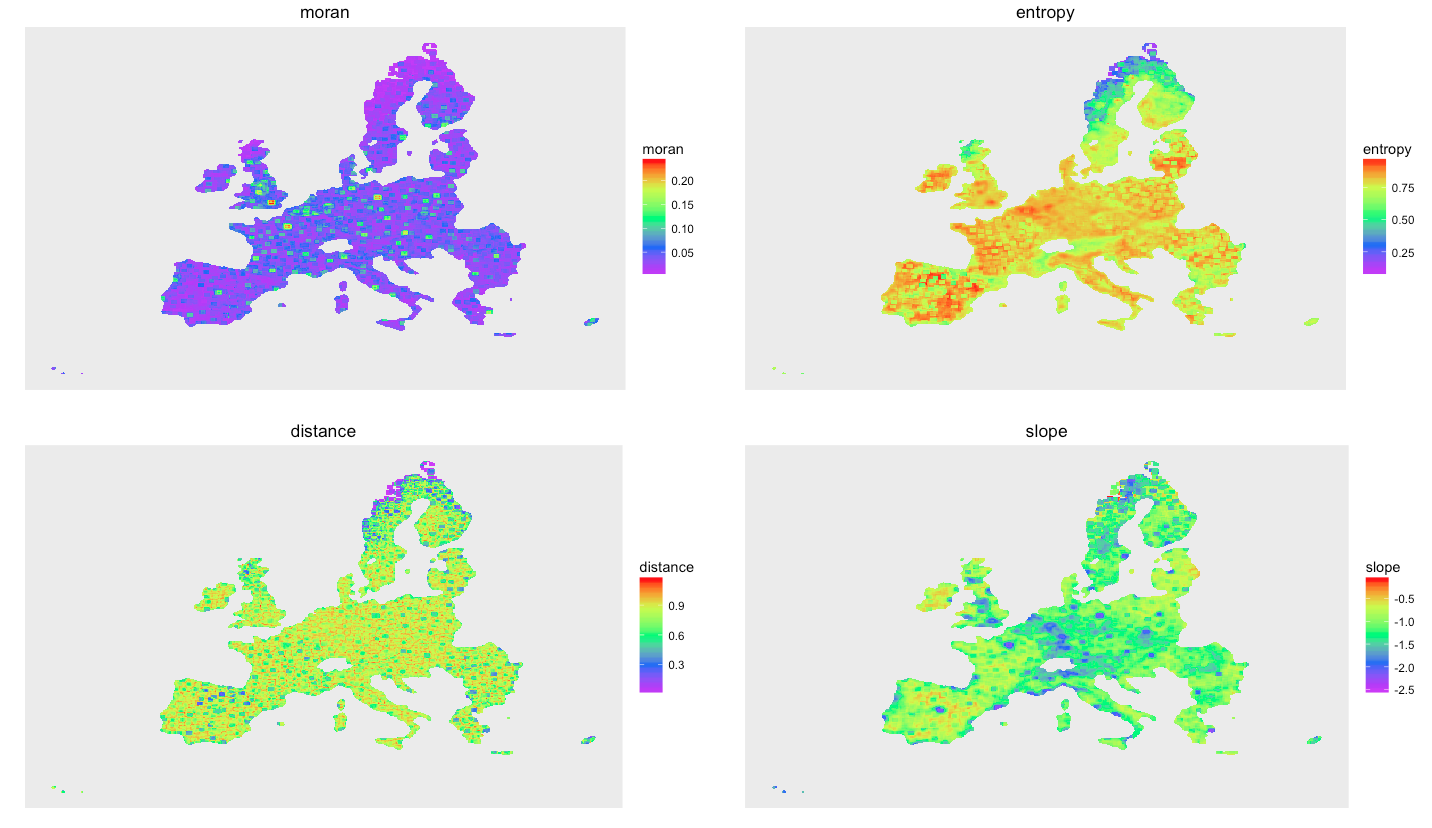
\includegraphics[angle=90,width=1.7\textwidth,height=\textheight]{Figures/PartII/Empirical/Static/Density/all_50km}
\caption[Geographical Distribution of Morphologies]{Geographical Distribution of Morphologies}
\end{figure}
%%%%%%%%%%%%%%%%%%


%%%%%%%%%%%%%%%%%%
\begin{figure}
\hspace{-3cm}
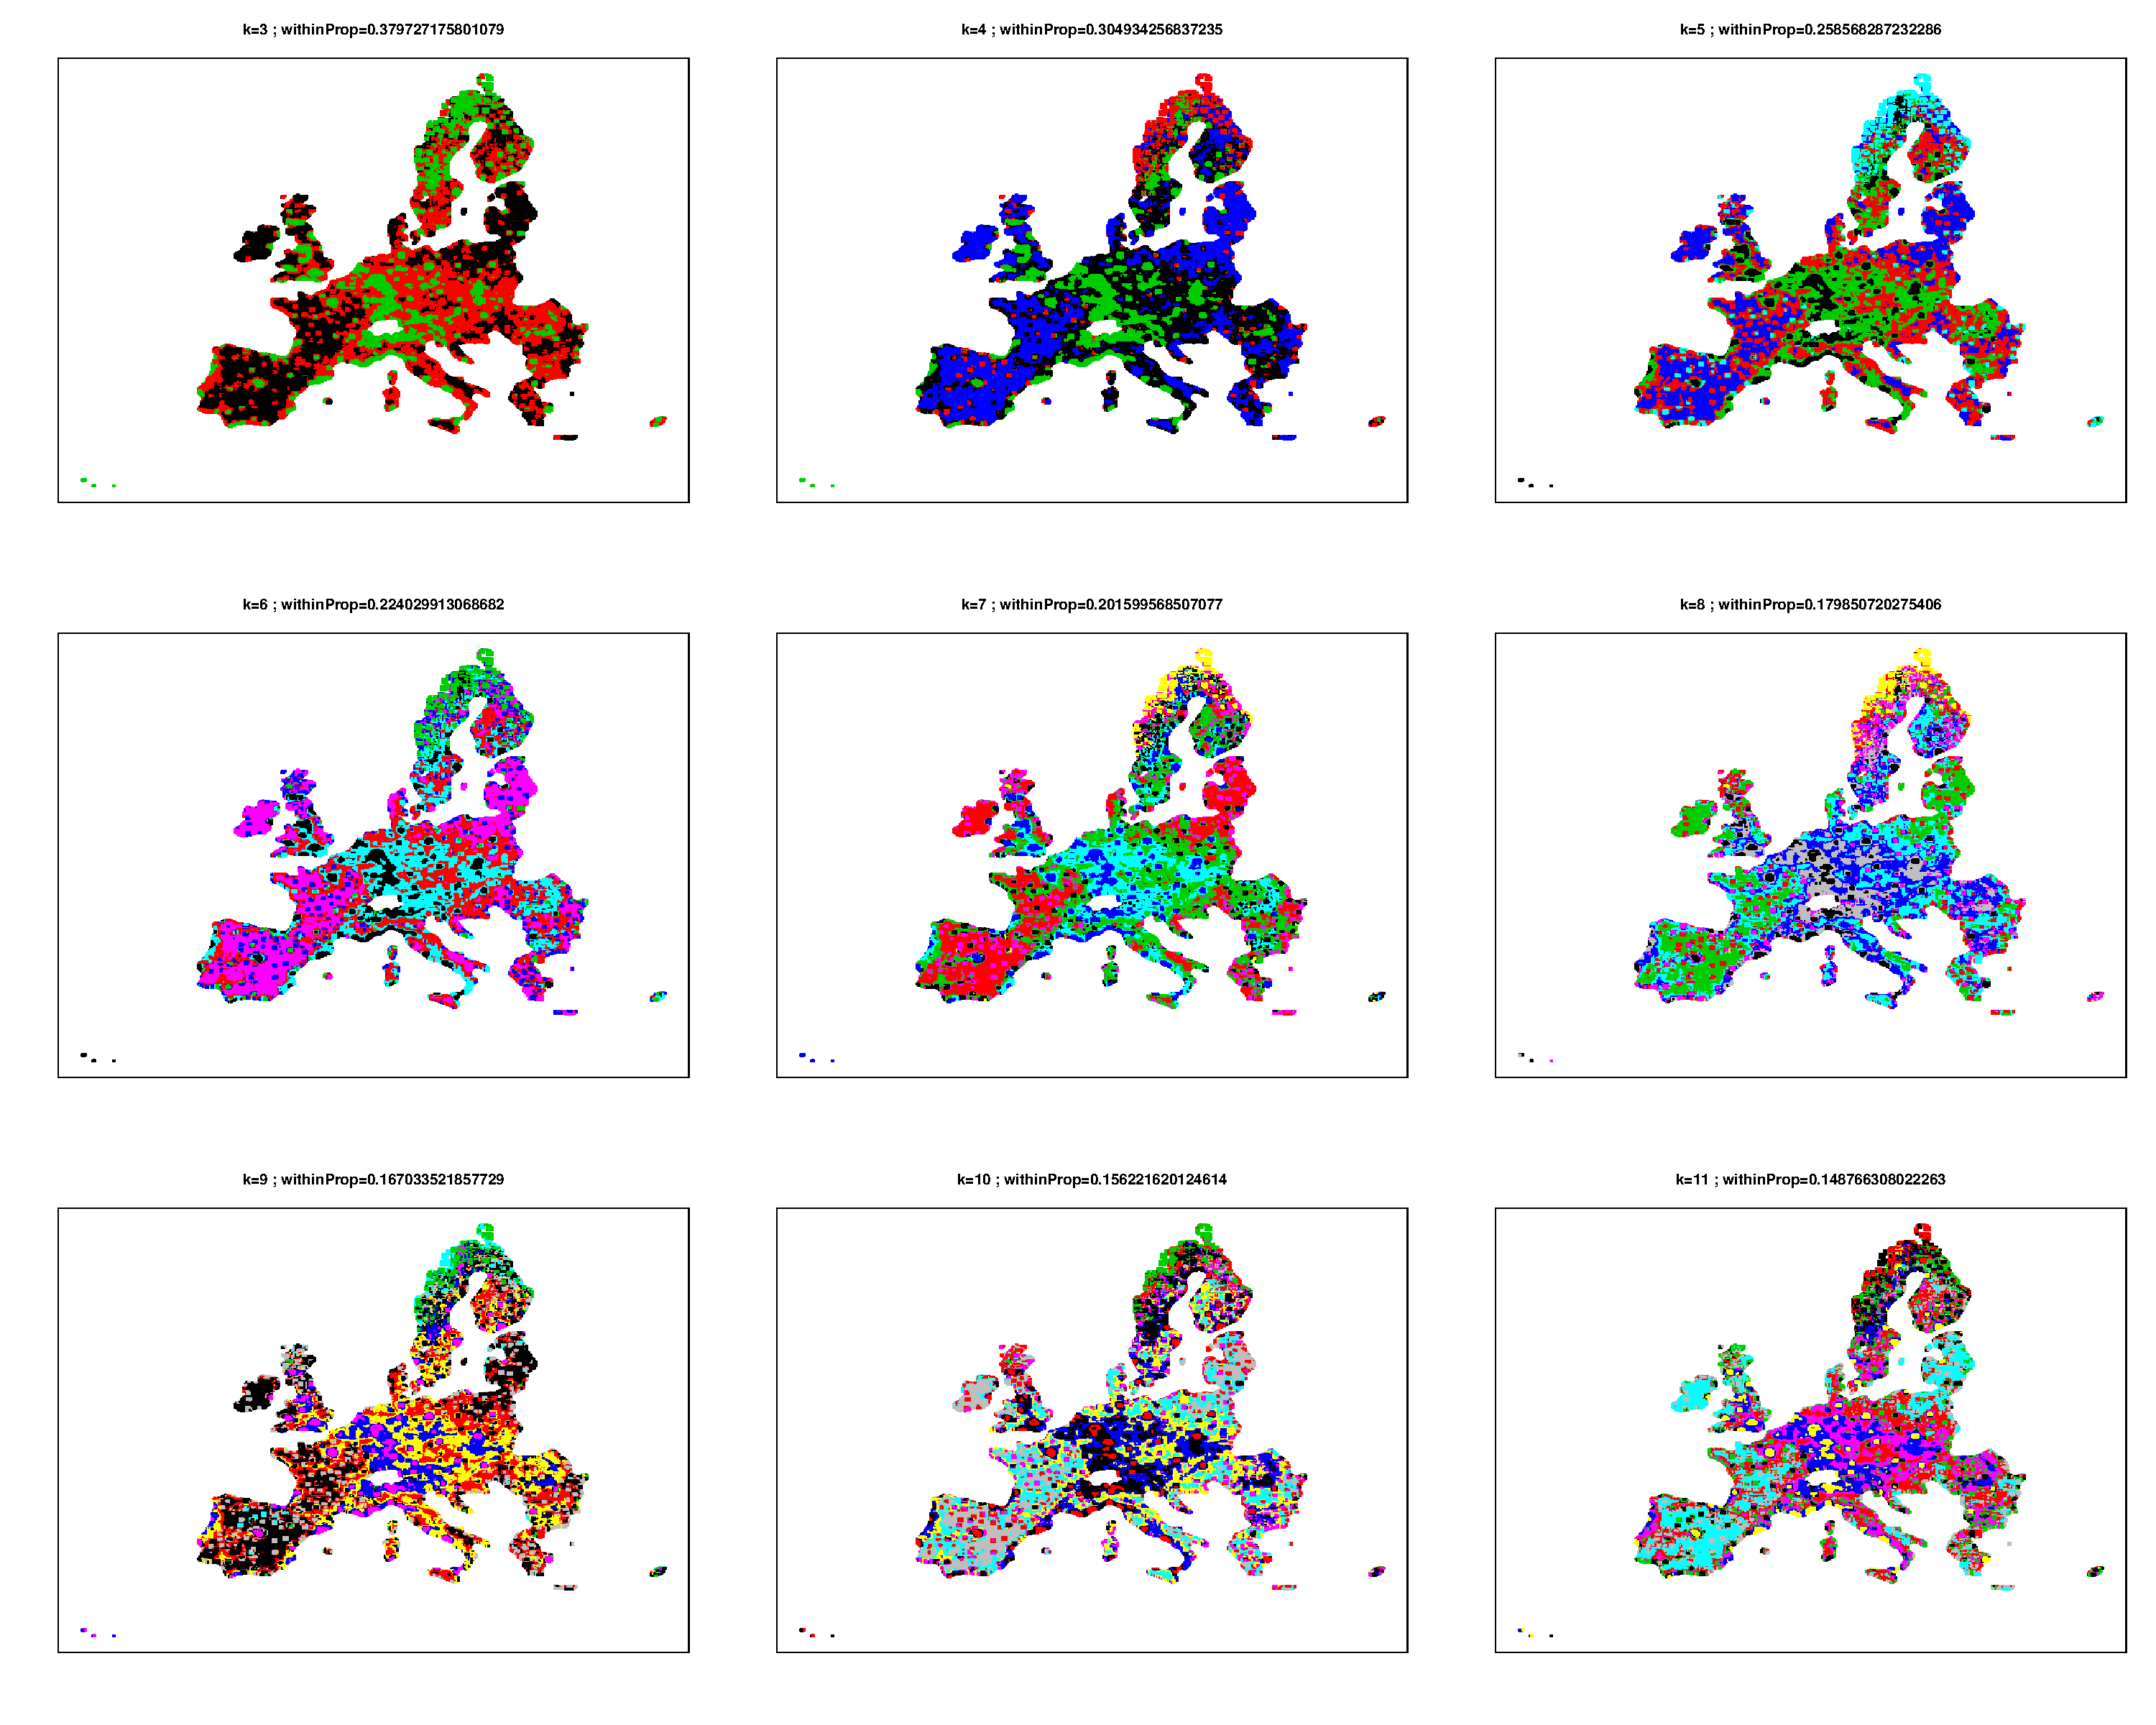
\includegraphics[angle=90,width=1.7\textwidth,height=\textheight]{Figures/PartII/Empirical/Static/Density/clust_k3-11}
\caption[Clustering Analysis of Morphologies]{Clustering Analysis of Morphologies}
\end{figure}
%%%%%%%%%%%%%%%%%%






\subsubsection{Further developments}

\cite{10.1371/journal.pone.0107042}

\url{http://www.worldpop.org.uk/}



%%%%%%%%%%%%%%%%%%
\subsection{Network Measures}

We consider network aggregated indicators as a way to characterize transportation network properties on a given territory, the same way morphological indicators yielded information on urban structure. We propose to compute some simple indicators on same extents as for morphology, to be able to explore relations between these static measures.

Network analysises : \cite{louf2014typology}


\subsubsection{Data preprocessing}

We work in a first time on road network, which structure is finely conditioned to territorial configuration of population densities. Furthermore, data for present day road network is available through the OpenStreetMap project~\cite{openstreetmap}. Its quality was investigated for different countries such as England~\cite{haklay2010good} and France~\cite{girres2010quality}. It was found to be of a quality equivalent to official surveys for the primary road network.

% data collected from http://download.geofabrik.de/europe.html


\paragraph{Simplification algorithm}

For a given dataset corresponding to a subset of the overall road network, it is necessary to simplify network structure by spatial aggregation as initial data presents very detailed features and thus a very large numbers of nodes ($\simeq 10^10$ for Europe dataset). Such a level of precision is not needed in our study since density data is already aggregated at 500m resolution. It is possible to drastically reduce network size by spatial aggregation of nodes and link replacements. More precisely we use the following procedure :
\begin{itemize}
\item a background raster (which resolution $r$ gives the snapping parameter for aggregation) is constructed from a reference raster and the extent of network. This grid gives spatial aggregation units for network nodes.
\item for each feature of the road dataset, corresponding connected raster cells are stored with corresponding impedance and distance in a sparse adjacency matrix.
\end{itemize}


\paragraph{Implementation}

A \texttt{PostGIS} database is used to store raw and simplified network, in order to perform efficient spatial requests, compared for example to initial \texttt{osm} data formats (\texttt{osm} or \texttt{pbf}). However


\paragraph{Sensitivity to simplification parameters}

% -> sensitivity to \theta_snap
% -> sensitivity to degree simplification (influence on means e.g.)


\subsubsection{Indicators}

Network macroscopic structure is summarized by the following set of indicators, after the simplifications and reductions done in the previous step. Assuming network given by $N=(V,E)$, nodes spatial positions $\vec{x}(V)$ and edges \emph{effective distances} $d(E)$ taking into account impedances and real distances (to include basically network hierarchy), we have indicators :
\begin{itemize}
\item connectivity
\item degree distribution
\item centrality, taken as normalized mean \emph{betweenness-centrality}
\item average path length
\item network diameter
\item mean network speed
\end{itemize}

These indicators are used to capture a rough picture of the structure. Refined work at smaller scales (intra-urban road network) and with more elaborated measures that allow to differentiate more precisely local form, was recently done by Lagesse in~\cite{2015arXiv151201268L}.



\subsubsection{Results}




%%%%%%%%%%%%%%%%%%
\subsection{Effective static correlations}



%%%%%%%%%%%%%%%%%%
\subsection{Insights for interaction processes}






%----------------------------------------------------------------------------------------


\newpage

\section{Disentangling co-evolutions from causal relations : a case study on \emph{Bassin Parisien}}


\cite{levinson2008density} % study on london with temporal and spatial lag (weird use of spatial statistics) -> expected conclusions but does not really disentangle ?



\subsection{Context Formalization}

\subsubsection{Variables}

\paragraph{Description}

We assume a dynamic transportation network $n(\vec{x},t)$ within a dynamic territorial landscape $\vec{T}(\vec{x},t)$, which components are to simplify population $p(\vec{x},t)$ and employments $e(\vec{x},t)$. Data is structured the following way :
\begin{itemize}
\item Observation of territorial variables are discretized in space and in time, i.e. the spatial field $\vec{T}$ is summarized by $\mathbf{T} = \left(\vec{T}(\vec{x}_i,t_j^{(T)})\right)_{i,j}$ with $1\leq i \leq N$ and $1\leq j \leq T$. They concretely correspond to census on administrative units (\emph{communes} in our case) at different dates.
\item Network has a continuous spatial position but
\end{itemize}



\paragraph{Definitions}



\subsection{On Accessibility}

% accessibility : need to introduce it ?
%  -> read Weibull

The notion of accessibility has been central to regional science since its introduction and systematization in planning around 1970. 

\paragraph{Existence of accessibility}

%An elegant axiomatic definition is derived in~\cite{weibull1976axiomatic}. Starting from expected properties of an accessibility function $A$ that associate a value to \emph{attraction} $a$ and distance $d$, defined on the set of discrete spatial configurations $\mathcal{C} = \cup_{n\in \mathbb{N}}{(d_i,a_i)_{1\leq i \leq n}}$. These properties include (among technical others with no thematic meaning) :
%\begin{enumerate}
%\item $A$ is invariant regarding the order of the configuration
%\item $A$ decrease with distance at fixed attraction and increase with attraction at fixed distance
%\item $A$ is invariant when adding null attractions and constant configurations
%\end{enumerate}

%A canonical decomposition of any accessibility function 




\textit{\textbf{Is the notion of accessibility crucial for statistical analysis ?}}

\medskip


Weibull has proposed an axiomatic approach to accessibility~\cite{weibull1976axiomatic}, deriving a canonical decomposition for any \emph{attraction-accessibility} function $A(a,d)$, assuming expected thematic axioms among others technical ones that are :
\begin{enumerate}
\item \footnotesize $A$ is invariant regarding the order of the configuration
\item \footnotesize $A$ decrease with distance at fixed attraction and increase with attraction at fixed distance
\item \footnotesize $A$ is invariant when adding null attractions and constant configurations
\end{enumerate}
Then $A$ verifies these \emph{iff} it is of the form
\[
A\left[(a_i,d_i)\right] = T\left(\bigoplus_i z(d_i,a_i)\right)
\]
where $T$ is increasing with null origin, $z$ is a \emph{distance substitution function} (i.e. verifying axiom 2) and $\oplus$ a \emph{standard composition} associating two attractions at zero distance to th corresponding unique one. 

$\rightarrow$ \textit{Well suited matrices of autocorrelation should capture accessibility in regressions ; or captured by non-linear regression on $\mathbf{N}$}

\medskip

{\normalsize\textit{\textbf{Accessibility as potential ?}}}

Given any stationary dynamic for $n,\vec{T}$, Helmoltz theorem states that it derives from a potential (can be adapted to non-stationary dynamics with time-varying potential).








\paragraph{Continuous approach and accessibility potential}

% Paul : Helmoltz-Hodge theorem to infer potential field from speed spatial field ?
%  Q : what are trajectories ? dirac field has no rotational -> continuous approach does not work ?






\subsection{Statistical Tests}



\textit{Large set of analysis to be tested (non exhaustive) :}
\begin{itemize}
\item On data :
\begin{itemize}
\item Multivariate models $\mathcal{L}\left[\mathbf{T},\mathbf{N}\right]\sim \varepsilon$
\item Autocorrelated univariate models $(\mathbf{I} - \Sigma R W) \mathbf{X} \sim \varepsilon$
\item Autocorrelated multivariate models $(\mathcal{L}' - \Sigma R W)\left[\mathbf{T}+\mathbf{N}\right] \sim \varepsilon$
\item Geographically Weighted Regression~\cite{brunsdon1998geographically}
\[
\mathcal{L}\left[\mathcal{G}\left(\mathbf{T},\mathbf{N}\right)\right] \sim \varepsilon
\]
\item Granger causality tests : \cite{xie2009streetcars} use Granger causality to link transit with land-use changes.
\end{itemize}
\item On data returns :
\begin{itemize}
\item Autoregressive multivariate models
\[\mathcal{L}\left[(\Delta \mathbf{T}(t_{j'}))_{j'\leq j},(\Delta \mathbf{N}(t_{j'}))_{j'\leq j}\right] \sim \varepsilon\]
\item Autoregressive autocorrelated multivariate models : idem with spatial autocorrelation term.
\item Synthetic Instrumental Variables : static territory and/or network ?
\end{itemize}
\end{itemize}



\subsubsection{Bivariate linear models}

\subsubsection{Autocorrelated univariate models}

\subsubsection{Autocorrelated multivariate models}

\subsubsection{Granger causality tests}

\cite{xie2009streetcars} use Granger causality to link transit with land-use changes.


\subsubsection{Autoregressive multivariate models}



\subsubsection{Autoregressive autocorrelated multivariate models}











%----------------------------------------------------------------------------------------

\newpage

\section{Early warnings of Network Breakdowns : socio-economic and real estate trajectories}


\subsection{Context}

Various aspects of territories are concerned by interactions with networks. In previous empirical studies, no socio-economic attributes of populations inhabiting the territory nor economic values for land and real estate was considered. Both are however crucial elements of territorial dynamics and are extensively studied in fields such as territorial analysis or urban economics : for example, \cite{homocianu:tel-00359302} studies households residential choices to understand land-use transportation interactions.

\cite{guerois2009dynamique} % results using base bien.


\subsection{Preliminary Results}



%%%%%%%%%%%%%%%
\begin{figure}
\hspace{-3cm}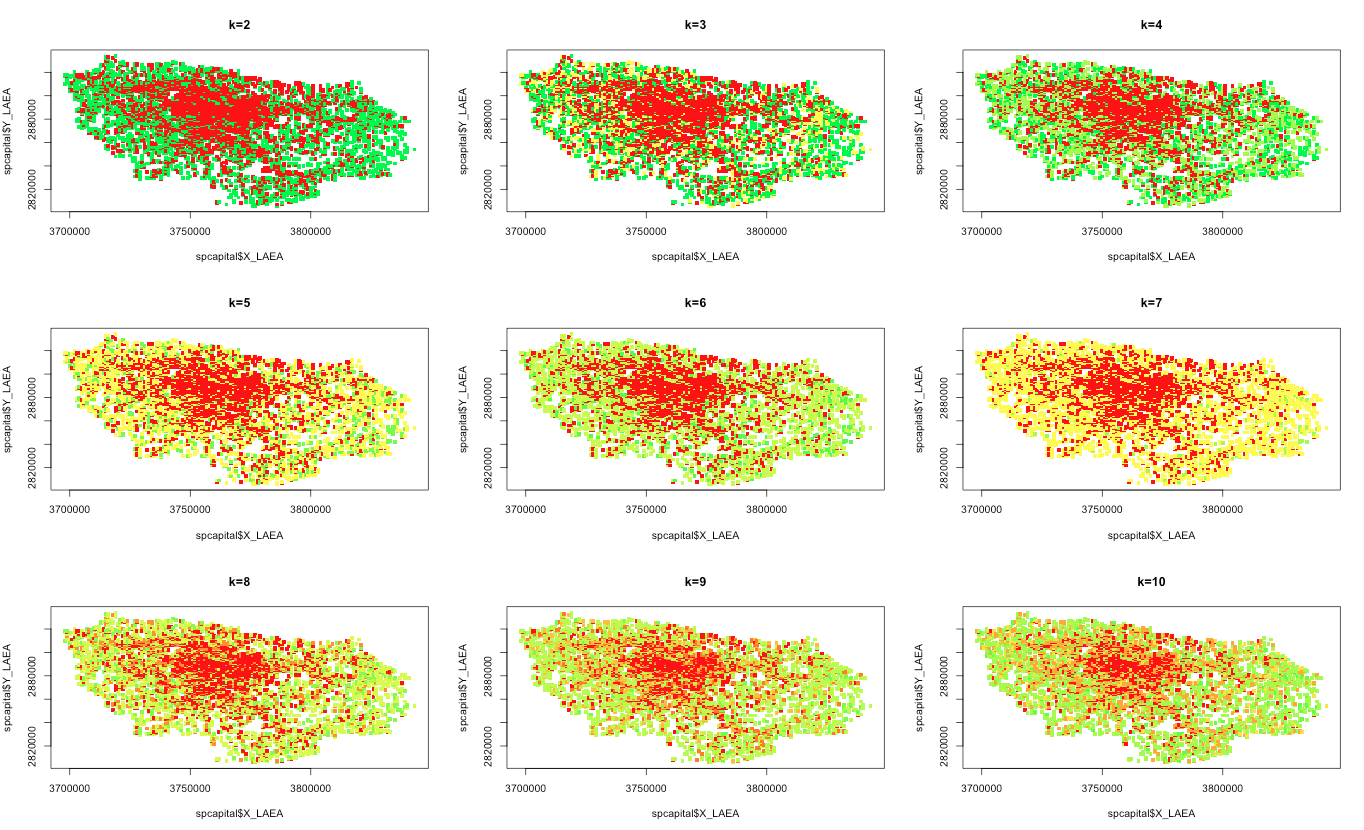
\includegraphics[width=1.4\textwidth]{Figures/PartII/Empirical/RealEstate/normalized_k2-10}
\smallskip
\hspace{-3cm}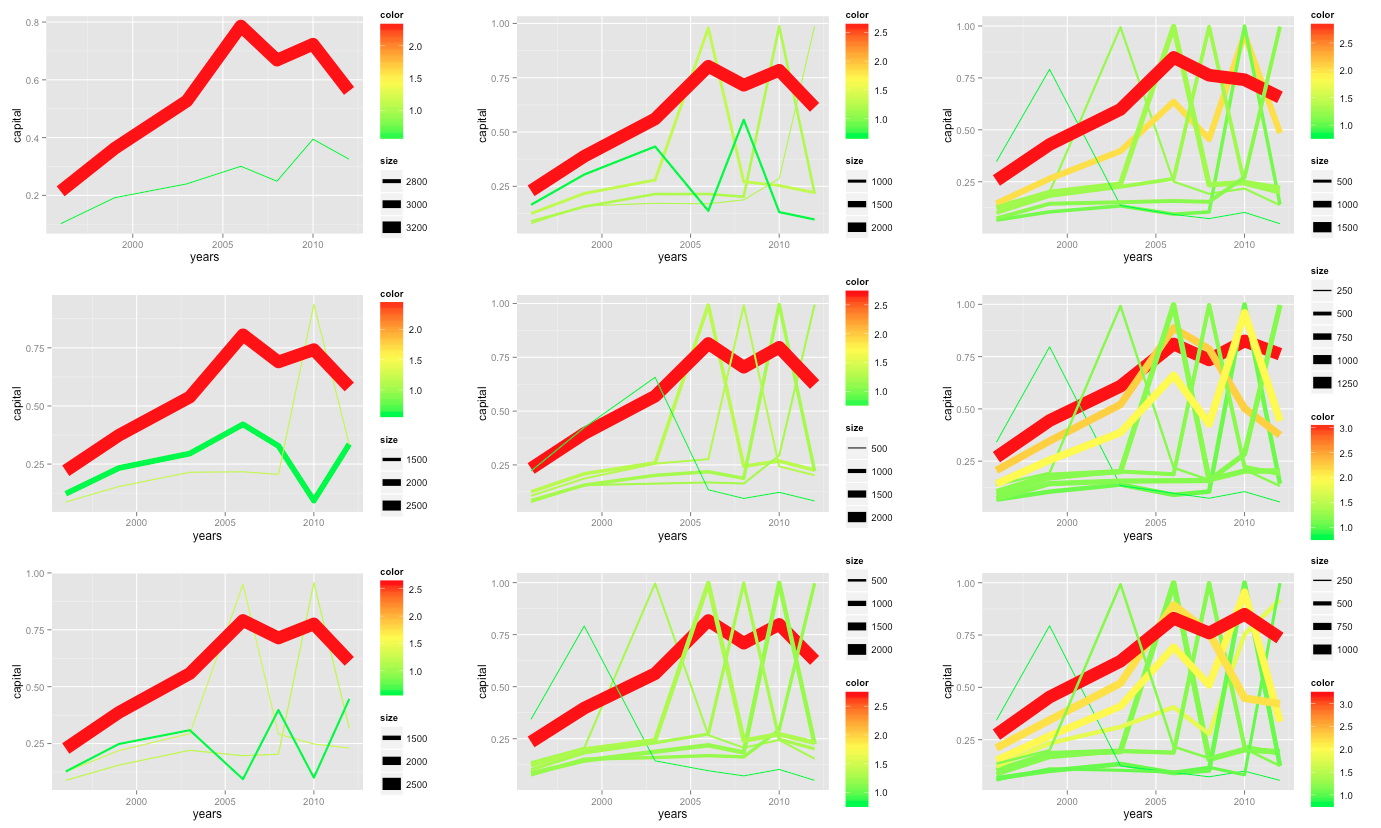
\includegraphics[width=1.4\textwidth]{Figures/PartII/Empirical/RealEstate/trajectories_normalized_k=2-10}
\caption[Typology of Real Estate trajectories]{Typology of Real Estate trajectories. Locations were categorized }
\end{figure}
%%%%%%%%%%%%%%%



\subsection{A strategy to investigate early warnings of network breakdowns}








%----------------------------------------------------------------------------------------

\newpage

\section[South-African historical events as instruments]{South-African historical events as instruments to understand network-territory relations}

The method of instruments in statistics is used to identify causal relationships between variables. We already identified the issue of causality in 







